% Copyright (C) Maximiliano Curia <maxy@gnuservers.com.ar>,
%               Margarita Manterola <marga@marga.com.ar>

% Esta obra está licenciada de forma dual, bajo las licencias Creative
% Commons:
%  * Atribución-Compartir Obras Derivadas Igual 2.5 Argentina
%    http://creativecommons.org/licenses/by-sa/2.5/ar/
%  * Atribución-Compartir Obras Derivadas Igual 3.0 Unported
%    http://creativecommons.org/licenses/by-sa/3.0/deed.es_AR.
%
% A su criterio, puede utilizar una u otra licencia, o las dos.
% Para ver una copia de las licencias, puede visitar los sitios
% mencionados, o enviar una carta a Creative Commons,
% 171 Second Street, Suite 300, San Francisco, California, 94105, USA.
\renewcommand{\chaptermark}[1]{\markboth{#1}{}}
\renewcommand{\thesection}{\arabic{section}}
\chapter*{Vectores y punteros}

Una particularidad de C, que puede parecer poco intuitiva al principiante, es
que al utilizar el nombre de una variable de un vector en nuestro código, C
(casi siempre)\footnote{Excepto para sizeof, \& y en el uso en la
inicialización de un vector en la declaración.} usa la dirección de memoria
donde está ubicado el vector.  Es decir, para prácticamente todos los usos, el
nombre de un vector es equivalente a un puntero.

El siguiente código imprime la posición de memoria del vector a:
\begin{codigo-c-plano}
  int a[] = {1, 2, 3, 4, 5};
  printf("%p\n", a);
\end{codigo-c-plano}

Por otro lado,

\begin{codigo-c-plano}
  int *p = a;
\end{codigo-c-plano}

Es una intrucción válida, ya que C guarda la dirección de memoria de a en p.
Sin embargo, esto no quiere decir que un vector sea un puntero.

\begin{figure}[htb]
\centering
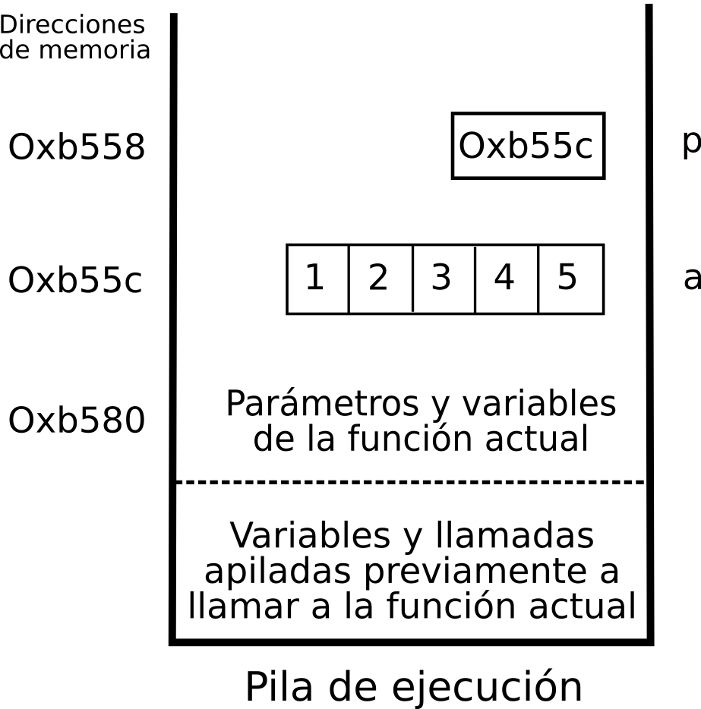
\includegraphics{imagenes/vectores-pila}
\caption{Pila de ejecución del código mostrado}
\end{figure}

Además de almacenarse de forma distinta en memoria, a un vector no se le puede
cambiar su posición en memoria, por lo que el siguiente código es inválido:

\begin{codigo-c-plano}
  int b[10];
  b = a; // ESTO NO ANDA
\end{codigo-c-plano}

En una función que recibe un arreglo por parámetro, en realidad C le pasa la
dirección de memoria del vector. Por ejemplo, si definimos la siguiente
función \lstinline!suma!:

\begin{codigo-c-plano}
  long suma(int *datos, int largo)
  {
    long res = 0;
    for(int i = 0; i<largo; i++) {
        res += datos[i];
    }
    return res;
  }
\end{codigo-c-plano}

El puntero \lstinline!datos! tendrá la dirección de memoria del vector recibido, 
\lstinline!datos! es un puntero y no un vector.  Para invocar a la función,
podremos hacerlo de la siguiente forma:

\begin{codigo-c-plano}
    suma(a, 5);
\end{codigo-c-plano}

Siendo \lstinline!a! el mismo vector con el que venimos trabajando. Al
poner el nombre del arreglo, C usa la dirección de memoria de \lstinline!a!
en la invocación a la función \lstinline!suma!.

En el código de \lstinline!suma! vemos que el puntero se usa exactamente
igual que como usaríamos el vector. Nuevamente, C usa la dirección del
arreglo (incluso para el operador \lstinline![i]!), por lo que el uso es
casi idéntico a utilizar un puntero.

En particular, el operador \lstinline!vector[posicion]! es exactamente lo
mismo que escribir \lstinline!*(vector+posicion)! y esto funciona ya que al
sumar un entero a una dirección de memoria el entero se multiplica por el
\lstinline!sizeof! del tipo apuntado (a esto último se lo suele llamar
\textit{aritmética de punteros}).

Para mayor claridad, el tipo de variable recibida (\lstinline!int *datos!)
se puede escribir también como \lstinline!int datos[]!, que es la forma
usual de recibir un vector en C.

\section{Vectores de vectores}

Al declarar cualquier tipo de vector, C requiere que cada posición del
vector tenga exactamente el mismo largo (en bytes), por lo que cada
posición debe ser de un tamaño fijo.

Es por ello que, si se desea armar un vector de vectores (una matriz), se
lo deba hacer de una forma particular.  Por ejemplo, si se desea construir
una matriz de 3 filas y 4 columnas, se lo podría hacer de la siguiente
manera:

\begin{codigo-c-plano}
    int v[][4] = {{1, 2, 3, 4}, {5, 6, 7, 8}, {9, 10, 11, 12}};
\end{codigo-c-plano}

Como se ve, es posible no especificar la cantidad de filas, ya que estas se
especificarán automáticamente al inicializar, pero  es imprescindible
especificar la cantidad de columnas, ya que esto es lo que determina la
medida de cada uno de los elementos del vector \lstinline!v!.

Para acceder a la información del vector, se lo hará de la forma intuitiva:
\lstinline!v[fila][columna]!.

Hasta aquí no resulta demasiado complejo.  Las limitaciones surgen cuando
se quiere poder pasar un vector por parámetro a una función.  La forma
correcta de pasar un vector como el mostrado a una función, sería la
siguiente:

\begin{codigo-c-plano}
void imprimir_matriz(int v[][4], size_t filas);
\end{codigo-c-plano}

Es decir que la cantidad de filas puede ser variable, y se la debe recibir
por parámetro, pero la cantidad de columnas es parte del tipo de la
variable, y se la debe indicar dentro de la declaración de la función.

Esto se debe a que los elementos en memoria se guardan uno a continuación
del otro, y C necesita saber cuántos elementos tiene cada una de las
filas para poder saber cuánto se tiene que desplazar hasta encontrar el
elemento.

\section{Usar un bloque contiguo de memoria como una matriz}

Una forma de poder hacer un manejo genérico de matrices en C es basarse en que
la matriz está guardada en forma contigua en memoria y hacer la cuenta de la
posición que le corresponde a cada elemento.

Siguiendo con el ejemplo anterior, \lstinline!v! como dirección de memoria
es la dirección del elemento \lstinline!v[0][0]!. En el siguiente espacio
dentro del bloque de la memoria, que se encuentra desplazado la cantidad de
bytes que mide un entero estará \lstinline!v[0][1]!. Desplazándose cuatro
veces ese tamaño tenemos \lstinline!v[1][0]!.

Utilizando esta idea, podemos crear una nueva variable \lstinline!x!, que sea
un puntero a enteros que apunta al comienzo de \lstinline!v!. Podemos utilizar
la \emph{aritmética de punteros} vista anteriormente: haciendo
\lstinline!(x + fila*cols)! (donde \lstinline!cols! es la cantidad de
elementos por fila) obtenemos la dirección del comienzo la fila
\lstinline!fila!, esta dirección es el comienzo de un vector de enteros, por
lo que podemos hacer \lstinline!(x + fila*cols)[columna]!, para acceder al
valor de \lstinline!v[fila][columna]!.

La ventaja que obtenemos al hacer esto es que podemos escribir funciones
genéricas, que reciban el tamaño de la matriz por parámetro. Por ejemplo:

\begin{codigo-c}
void imprimir_matriz(void* aux, size_t filas, size_t cols)
{
    int *x = aux;
    for (int i=0; i < filas; i++) {
        for (int j=0; j < cols; j++) {
            printf("%d ", (x + i*cols)[j]);
        }
        printf("\n");
    }
}
\end{codigo-c}

Y la invocación a esta función sería \lstinline!imprimir_matriz(v, 3, 4)!

\section{Vectores de vectores de tamaño variable}

Teniendo en cuenta lo visto anteriormente, si se quiere crear matrices
cuyas columnas sean variables como las filas, que se las pueda pasar por
parámetro a funciones sin importar cuántas columnas tenga, será necesario
recurrir a la memoria dinámica.

Para el caso anterior, por ejemplo, se podría declarar un vector de
punteros, y cada uno de esos vectores inicializarlo como un vector de
enteros:

\begin{codigo-c-plano}
    int *w[filas];
    for (int i=0; i < filas; i++) {
        w[i] = malloc(cols*sizeof(int));
    }
\end{codigo-c-plano}

En este código, \lstinline!w! es un vector de \lstinline!filas! punteros.
Cada uno de estos punteros contiene la dirección de memoria de una porción
de memoria dinámica de tamaño \lstinline!cols*sizeof(int)!.

Al pasar este vector por parámetro a una función, se lo hará de la
siguiente manera:

\begin{codigo-c-plano}
void imprimir_matriz(int** v, size_t filas, size_t cols) {
\end{codigo-c-plano}

Utilizando este formato será posible seguir accediendo a los datos
contenidos en la matriz como \lstinline!v[fila][columna]!.

\begin{figure}[htb]
\centering
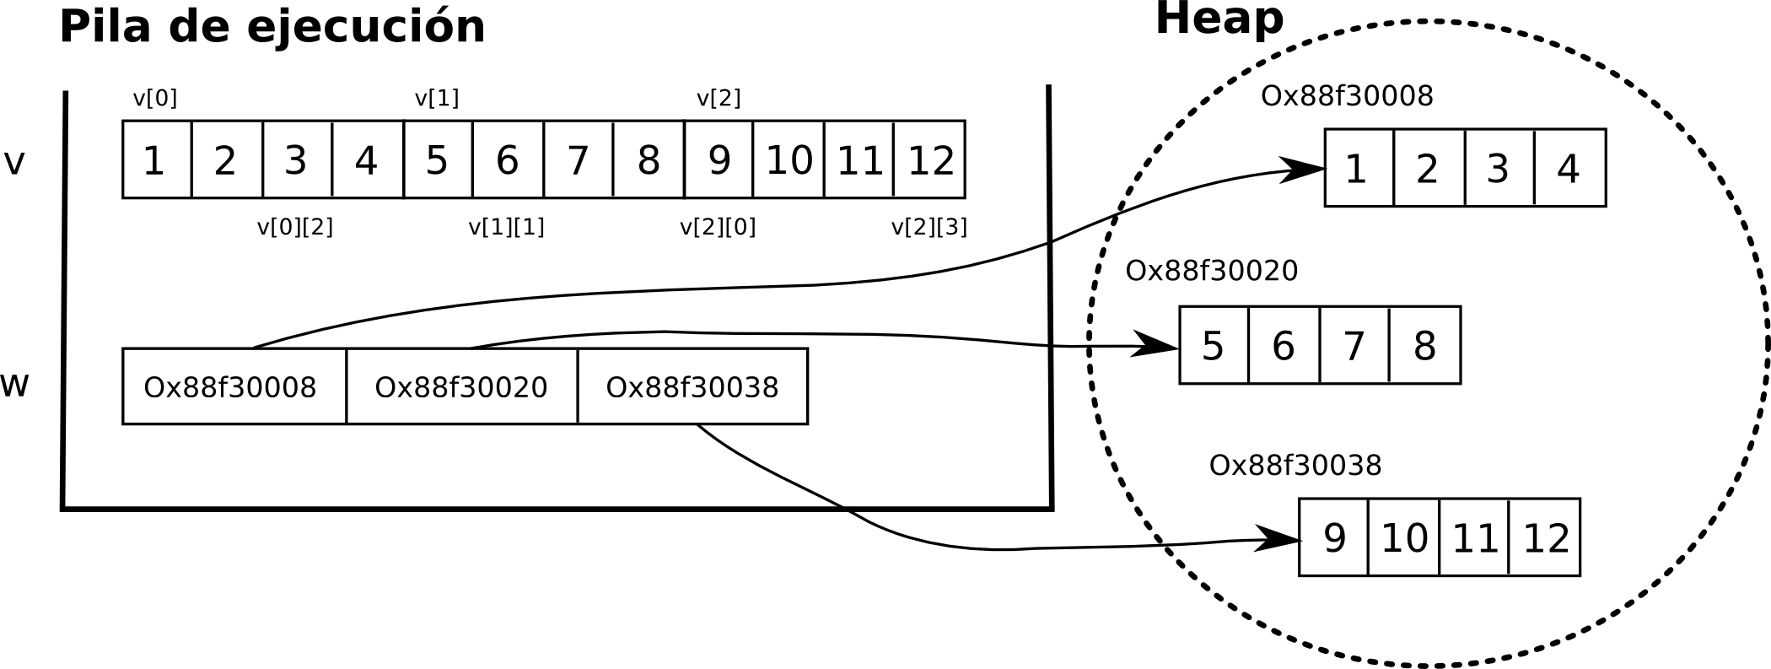
\includegraphics{imagenes/vectores-matrices}
\caption{Ubicación de los vectores mostrados en la memoria}
\end{figure}

\section{Cadenas y vectores de cadenas}

Como ya se ha mencionado, las cadenas en C son arreglos de caracteres,
terminados por un caracter \lstinline!\0!.

Si bien es posible declararlas como \lstinline!char cadena[largo]!, lo más
usual es declararlas como \lstinline!char *cadena! y luego asignar una
dirección de memoria apropiada para el dato que se quiera representar.

Cuando se declara una cadena en memoria estática, como en el siguiente
ejemplo:

\begin{codigo-c-plano}
char *cadena = "Algoritmos";
\end{codigo-c-plano}

La variable \lstinline!cadena! contiene una dirección de memoria, en la
cual comienza el arreglo de caracteres, que tiene 11 caracteres (10 letras
y un \lstinline!\0! al final). \\

Si se quiere tener un arreglo que contenga varias cadenas, se deberá operar
de manera similar a la mostrada para las matrices.

\begin{codigo-c-plano}
    char* palabras[] = {"Hola", "que", "tal"};
\end{codigo-c-plano}

Es decir que en este caso la variable \lstinline!palabras! contiene un
arreglo de tres punteros, cada uno de los cuales apunta a una porción de
memoria donde están almacenadas las palabras.

